
\documentclass[12pt]{article} % use larger type; default would be 10pt

\usepackage[utf8]{inputenc} % set input encoding (not needed with XeLaTeX)

%%% PAGE DIMENSIONS
\usepackage{geometry} % to change the page dimensions
\geometry{a4paper} % or letterpaper (US) or a5paper or....
\geometry{margin=1in} % for example, change the margins to 2 inches all round
% \geometry{landscape} % set up the page for landscape
%   read geometry.pdf for detailed page layout information

\usepackage{graphicx} % support the \includegraphics command and options

% \usepackage[parfill]{parskip} % Activate to begin paragraphs with an empty line rather than an indent

%%% PACKAGES
\usepackage{booktabs} % for much better looking tables
\usepackage{array} % for better arrays (eg matrices) in maths
\usepackage{paralist} % very flexible & customisable lists (eg. enumerate/itemize, etc.)
\usepackage{verbatim} % adds environment for commenting out blocks of text & for better verbatim
\usepackage{subfig} % make it possible to include more than one captioned figure/table in a single float
% These packages are all incorporated in the memoir class to one degree or another...

%%% HEADERS & FOOTERS
\usepackage{fancyhdr} % This should be set AFTER setting up the page geometry
\pagestyle{fancy} % options: empty , plain , fancy
\renewcommand{\headrulewidth}{0pt} % customise the layout...
\lhead{CS 5150 Milestone 3 Report}\chead{}\rhead{Sun in the City Group}
\lfoot{}\cfoot{\thepage}\rfoot{}

%%% SECTION TITLE APPEARANCE
\usepackage{sectsty}
\allsectionsfont{\sffamily\mdseries\upshape} % (See the fntguide.pdf for font help)
% (This matches ConTeXt defaults)

%%% ToC (table of contents) APPEARANCE
\usepackage[nottoc,notlof,notlot]{tocbibind} % Put the bibliography in the ToC
\usepackage[titles,subfigure]{tocloft} % Alter the style of the Table of Contents
\renewcommand{\cftsecfont}{\rmfamily\mdseries\upshape}
\renewcommand{\cftsecpagefont}{\rmfamily\mdseries\upshape} % No bold!

%%% END Article customizations

%%% The "real" document content comes below...

\title{CS 5150 Milestone 3 Report \\ Sun in the City Group}
\author{Phillip Tischler (pmt43), Brian Toth (bdt25), Vera Khovanskaya (vdk9), \\ 
Sean Salmon (ss2669), Lin Xue (lx39), Zach Porges (zip2),  \\
and James McGuinness (jrm369)}
%\date{} % Activate to display a given date or no date (if empty),
         % otherwise the current date is printed 

\begin{document}
\maketitle
\tableofcontents
\clearpage

%%%%%%%%%%%%%%%%%%%%%%%%%%%%%%%%%%%%%%%%%%%%%%%%%%%%%%%%%%%%%%%%%%%%%%%%%%%%%%%%
\section{Milestone Summary}

TODO

%%%%%%%%%%%%%%%%%%%%%%%%%%%%%%%%%%%%%%%%%%%%%%%%%%%%%%%%%%%%%%%%%%%%%%%%%%%%%%%%
\section{Project Description}

The goal of the project is to create a new website and Content Management System (CMS) for the Cornell Daily Sun in a new market: Cornell’s new Tech Campus in New York City. According to the client, Joseph Staehle, IT Manager for the Daily Sun, it should be a ``Totally online, totally tech based newspaper for the tech campus.”

The website is being built using Drupal, but will involve a custom front-end design as well as intelligent back-end technology. The website will include data fusion, aggregation of articles from other news sources.

%%%%%%%%%%%%%%%%%%%%%%%%%%%%%%%%%%%%%%%%%%%%
\subsection{Scope \& Requirements}

The project analyzed in this document is one to build a new website and Content Management System (CMS) for The Cornell Daily Sun. This website will represent a new market for the client. That is, the client is attempting to expand its newspaper to begin bringing news to the students of Cornell University’s new Tech Campus in New York City.
                   
\subsubsection{System Status}
                   
The Cornell Daily Sun website is an existing product that is managed with a Drupal CMS and custom extensions. This project is to build a new website for the Cornell Tech Campus, and is therefore a new product and not an augmentation or replacement. However, if this new website is extremely successful the old website may be converted to the new one. To maintain familiarity with the CMS system, the client has requested the CMS be based on the Drupal CMS.
                   
\subsubsection{Functionality}
                   
There are four required pieces of functionality the project must support: a website for readers to browse the newspaper, a CMS to manage the website and allow writers to post content, a means to allow Data Fusion to present external content inline with content generated by The Cornell Daily Sun, and finally a Brand to associate with this new website. Like the existing CMS The Cornell Daily Sun uses, the CMS must allow the writers and editors to upload their content like articles, blogs, comments, images, and advertisements. The website itself must display this content in a reasonable and convenient way that allows readers to browse and obtain the information they are looking for. To create a unique Cornell Tech campus newspaper, the project also requires the team to create a Brand. This includes a logo, a display name, and a look and feel for this newspaper. A key aspect of this Brand will be Data Fusion, a distinction from the current website the client operates. Data Fusion will present articles from external sources inline with an article posted by the Cornell Daily Sun. It is similar to a ``Read More" link, except this information will be external and automatically presented with the article from The Cornell Daily Sun.
                   
There are three desired but not required pieces of functionality for the project: an optimized mobile version of the site, an algorithm to perform the Data Fusion automatically, and a performance optimizer for the entire system. The mobile optimized site will allow readers to browse The Cornell Daily Sun’s website on a mobile device in a much faster and convenient way than to load the main page onto a slower device with less screen display area. This functionality may require too much time to implement, which is why it is not a required portion of this project. The Data Fusion described in the paragraph above was a framework to allow custom algorithms to link external content as well as manually link content. The other piece of functionality that is not required is an algorithm to automatically detect and link external content to the content generated by The Cornell Daily Sun. This may involve web and RSS feed scraping as well as Machine Learning and other advanced topics. Due to the complexity of the functionality relative to the timeframe of the project, this functionality has been deemed not required. However, if implemented it will save time, make running the website easier, and increase the attractiveness to potential readers as it will dynamically update the site. The final desired but optional piece of functionality is a performance optimization that will decrease the time it takes to load the website. Using a 50Mbps connection (an average user only has access to a 2Mbps connection), the client’s current site takes over 5 seconds to load the visible page of the homepage and over 13 seconds to load the entire page. Most websites can respond in under 200 milliseconds and load completely in a second. Every millisecond the user waits has a psychological impact on their perception of the website, and thus it is critical to load as fast as possible. There are simple upgrades to the system that can be employed to achieve this goal. However, time and budget may be a limiting factor, which is why this functionality is desired but not required.

\subsubsection{Dependencies}
                   
Drupal. Drupal is an open-source CMS that The Cornell Daily Sun uses for their current website, and as such the CMS that will be used for this project. The Drupal CMS is licensed under the GNU General Public License. This license is explained under the discussion of business considerations. Drupal is composed PHP, HTML, and CSS to generate and display the content, and a MySQL database to store the information composing the content itself. Drupal 6 requires PHP 4.4.0 or higher, while Drupal 7, the latest release, will be used and it requires PHP 5.2.5. Drupal provides a large baseline of features for a website, including but not limited to, user account handling, layout management, website menu customization, RSS feed aggregation, article search, and FTP access. Extensions can be written for Drupal in PHP, and there are over 17,000 free extensions available that are also under the GNU General Public License. For this project, Drupal will provide a very strong base for building this system.
Deployment Server. We will be using a Linux-based server hosted on a cloud platform for purposes of development and eventually deployment. The plan is to use Amazon AWS as the cloud provider. Because Drupal uses PHP and MySQL only, a Linux server is appropriate.
Data Fusion. The Data Fusion extension will most likely be integrated into Drupal using a PHP module, but the core functionality of the scraper will be written in Java. Because Drupal already has RSS aggregation, it is very likely that the module will rely on some form of RSS news scraping to find similar news articles.
Apache Lucene. The Data Fusion algorithm will be using the Apache Lucene indexing and search library that is licensed under the Apache 2.0 license. This license has been vetted and determined appropriate for this project.
                    

%%%%%%%%%%%%%%%%%%%%%%%%%%%%%%%%%%%%%%%%%%%%
\subsection{Benefits}

There are two unique stakeholder entities that will benefit this project. The first is The Cornell Daily Sun that will own the product that results from the project. The second is the students and other community members of Cornell University’s new Tech Campus. Each entity will benefit in different ways from the success of this project.
                   
\subsubsection{Cornell Daily Sun}
                   
With the new website, The Cornell Daily Sun will both expand its market, increase its influence, and increase its revenue. This project will allow the client to new types of content for both its paper based and web based publications. As the website matures, the project will allow the client to attract new readers on the order of 80,000. As the website displays advertisements, there will be a new source of income for the Cornell Daily Sun. Finally, with the new content and new readers in the New York City area, the website is very likely to attract new advertisers.
                   
Another potential benefit of the project is the integration of new technology. That is, the current website the client runs is on an older Drupal 6 CMS whereas the new website will be built with Drupal 7. Our new design will better organize the website content, and eciency code will be used to improve the compiling time from minutes to seconds. The Drupal 7 has major improvements over the Drupal 6. They are enhanced security (for scheduled tasks, password, and log-in), usability (better support for both administrators and users), and performance (new features for search, file handling, and RSS feeds). These new technical improvements are desired in the current Cornell Daily Sun website. If this project is a success, it can be deployed to replace the current website as well.
                   
\subsubsection{The Cornell Tech Campus Community}
                   
The website to be developed provides a way for broadcasting current news about the Cornell NYC Tech campus, which serves the Tech campus members and the general Cornell community. With blog services in addition to news, the website also enables individuals to share information with the community about tech topics, their life, campus life, alumni activity, and career experience. 

%%%%%%%%%%%%%%%%%%%%%%%%%%%%%%%%%%%%%%%%%%%%%%%%%%%%%%%%%%%%%%%%%%%%%%%%%%%%%%%%
\section{System Design}

The system has been designed to be as modular and uncoupled as possible. The Cornell Daily Sun’s current website is highly coupled and has prevented them from upgrading their system form Drupal 6 to Drupal 7.

The website will be hosted on Amazon AWS running an Apache 2 Web Server and a MySQL Database Server. Drupal 7 will be used to provided the base CMS and website structure. The team will develop custom XHTML, CSS, and PHP to create a ``theme" in Drupal. This customization can easily be ported to other Drupal versions and is a lightweight display layer. This will generate the viewable site and handle HTTP requests.

\begin{figure}[htbp]
\begin{center}
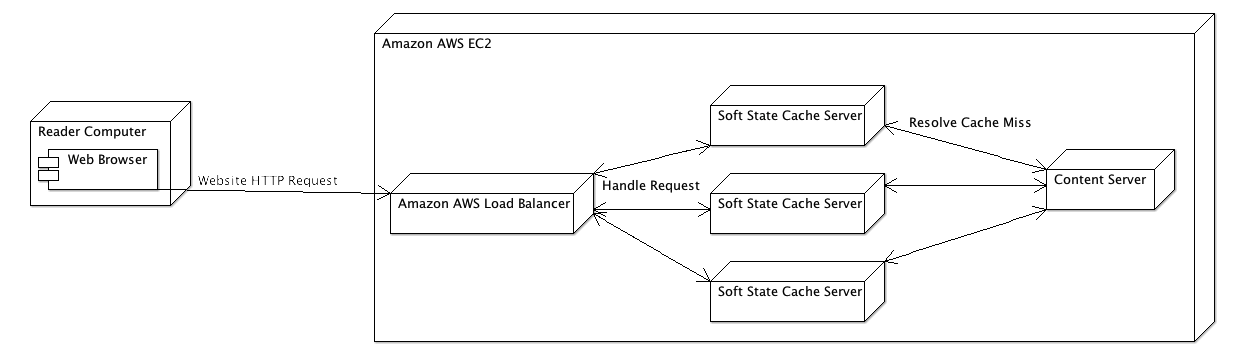
\includegraphics[width=6in]{images/data_flow}
\caption{Deployment Diagram}
\end{center}
\end{figure}

A Varnish server will be used as a soft-state in memory cache server. It works as a reverse proxy HTTP server and can handle about 3,000 page requests a second. This will provide incredible performance and scalability of the new site. Drupal also has pre existing modules to integrate with Varnish. This allows Drupal to invalidate page cache entries as the website is updated by The Cornell Daily Sun and happens completely behind the scenes.

Java will be used for the Data Fusion algorithm. The first component is RSS and Website Feed scraping. Various libraries are being analyzed to handle this workload. Essentially, the program will listen to RSS feeds and store the data in a MySQL database. Another component, the indexer, will take the data that has been scraped and put it into an Apache Lucene Index. Finally another component, the data fusion algorithm, will use the meta-tag taxonomy of an article to search for relevant data in the RSS and Website Apache Lucene Index, and store likely matches in another MySQL table.

To choose which Data Fusion articles get posted on the website, the team will build a lightweight PHP Drupal Extension to allow editors to approve fusion results as well as add in manual fusion data. This module will be an extremely lightweight and as decoupled as possible.

\begin{figure}[htbp]
\begin{center}
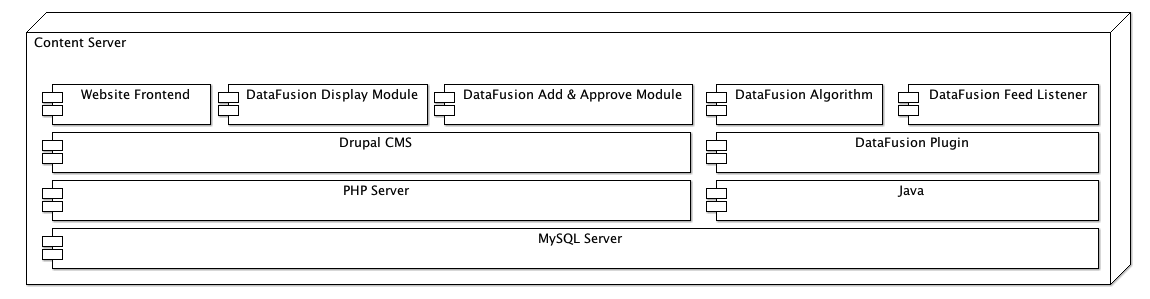
\includegraphics[width=6in]{images/software_stack}
\caption{System Architecture}
\end{center}
\end{figure}

%%%%%%%%%%%%%%%%%%%%%%%%%%%%%%%%%%%%%%%%%%%%%%%%%%%%%%%%%%%%%%%%%%%%%%%%%%%%%%%%
\section{Progress for Milestone 3}

TODO

%%%%%%%%%%%%%%%%%%%%%%%%%%%%%%%%%%%%%%%%%%%%%%%%%%%%%%%%%%%%%%%%%%%%%%%%%%%%%%%%
\section{Planning}

TODO

%%%%%%%%%%%%%%%%%%%%%%%%%%%%%%%%%%%%%%%%%%%%%%%%%%%%%%%%%%%%%%%%%%%%%%%%%%%%%%%%
\section{Issues Arisen}

TODO

%%%%%%%%%%%%%%%%%%%%%%%%%%%%%%%%%%%%%%%%%%%%%%%%%%%%%%%%%%%%%%%%%%%%%%%%%%%%%%%%
\section{Preliminary Documentation}

TODO

\begin{itemize}
\item https://help.ubuntu.com/community/ApacheMySQLPHP
\item http://drupal.org/documentation
\item http://lucene.apache.org/core/4\_0\_0/index.html
\item https://www.varnish-cache.org/docs
\end{itemize}

\end{document}
